\documentclass[a4paper,12pt]{article}
\usepackage[french]{babel}
\usepackage[utf8]{inputenc}
\usepackage[T1]{fontenc}
\usepackage{geometry}
\usepackage{graphicx}
\usepackage[colorlinks=true, linkcolor=blue, urlcolor=blue, citecolor=blue]{hyperref}
\usepackage{amsmath, amssymb}
\usepackage{float}

\geometry{margin=2.5cm}

\title{Projet : Implémentation du Jeu de la Vie en JavaFX}
\author{AMOUSSOU Mensanh Boris \\
L2, Groupe 2B Informatique – Université de Caen}
\date{\today}

\begin{document}

\maketitle
\tableofcontents
\newpage
    \section{Introduction}
    \subsection{Description générale du projet}
    Le Jeu de la Vie est un automate cellulaire inventé par le mathématicien britannique John Horton Conway en 1970. Il s'agit d'un modèle qui simule la vie d'un ensemble de cellules selon des règles simples. Chaque cellule peut être soit vivante, soit morte, et son état évolue au cours du temps en fonction du nombre de ses voisins vivants. Le projet consiste à implémenter cette simulation sous forme d'une interface graphique utilisant JavaFX, permettant à l'utilisateur d'interagir avec la grille et de voir l'évolution des cellules au fil du temps.
    \subsection{Identification de la problématique}
    La principale problématique réside dans l'implémentation des règles du jeu et l'interaction avec l'interface graphique. En effet, il est nécessaire de bien gérer l'évolution de la grille. La mise à jour de la grille doit être rapide tout en respectant les règles de John Conway. 
\section{Structuration du projet}
\subsection{Description des besoins du projet}
Le projet nécessite la création d'une grille de cellules, avec la possibilité de définir l'état initial des cellules (vivantes ou mortes). La grille doit évoluer selon les règles du Jeu de la Vie, mises à jour régulieres. Une interface graphique pour afficher cette grille et permettre à l'utilisateur d'interagir avec elle.
\subsection{Fonctionnalités implémentées}
Les principales fonctionnalités implémentées sont les suivantes :
\begin{enumerate}
    \item \textbf{Initialisation de la grille :} 
    La grille est initialisée avec des cellules mortes, et l'utilisateur peut activer ou désactiver certaines cellules pour définir l'état initial.\\
    \item \textbf{Simulation du jeu :} 
   L'état de la grille évolue en fonction des règles du Jeu de la Vie (comptage des voisins et application des règles de 
 John Conway).\\
   \item \textbf{Interface utilisateur :} 
  Une interface graphique permet de visualiser la grille et d'interagir avec elle.\\
  \item \textbf{Animation :} 
  L'évolution de la grille est animée à l'aide de la classe Timeline de JavaFX, avec un intervalle de mise à jour prédéfini à 500 ms.
\end{enumerate}
\subsection{Organisation du projet}
Le projet a été divisé en trois classes principales :
\begin{enumerate}
    \item \textbf{JeuDeLaVieModel :} 
    Gère la logique du jeu, y compris les calculs des voisins et cellules vivantes.\\
    \item \textbf{MaGrilleView :} 
   Gère l'affichage de la grille et l'interface graphique.\\
   \item \textbf{MaGrilleController :} 
  Gère l'interaction entre JeuDeLaVieModel et MaGrilleView, en contrôlant le déroulement de la simulation.
\end{enumerate}
\section{Éléments techniques}
\subsection{Description des structures de données}
La grille est un tableau à deux dimensions contenant des objets(cellules) de type Color[][], où chaque cellule peut être soit vivante (représentée par la couleur verte), soit morte (représentée par la couleur beige). La grille est de taille fixe (par défaut 25x25), mais cette taille peut être modifiée.
\subsection{Description des algorithmes}
Les algorithmes principaux du projet sont :
\begin{enumerate}
    \item \textbf{Calcul des voisins vivants :}
    Pour chaque cellule, on compte le nombre de cellules voisines vivantes en tenant compte de la grille cyclique (les bords se rejoignent). Cet algorithme est implémenté dans la méthode \fbox{compterVoisin} dans la classe JeuDeLaVieModel.
    \begin{figure}[H]
        \centering
        \includegraphics[width=0.9\linewidth]{compterVoisin.png}
        \caption{implémentation de la méthode compterVoisin}
    \end{figure}
    \item \textbf{Mise à jour de la grille :} À chaque génération, l'état de chaque cellule est mis à jour en fonction des règles du jeu (sous-population, sur-population, reproduction). Cette opération est réalisée dans la méthode \fbox{MiseAJour} dans la classe MaGrilleView.
     \begin{figure}[H]
        \centering
        \includegraphics[width=0.9\linewidth]{MAJ.png}
        \caption{une partie de la méthode MiseAJour}
    \end{figure}
    \item \textbf{Nombre de cellules vivantes :} À chaque génération, le nombre de cellules vivantes est compté. Cette opération est réalisée dans la méthode \fbox{celluleVivante} dans la classe JeuDeLaVieModel.
     \begin{figure}[H]
        \centering
        \includegraphics[width=0.9\linewidth]{celluleVivante.png}
        \caption{implémentation de la méthode celluleVivante}
    \end{figure}
    \end{enumerate}
    \section{Architecture du projet}
    \subsection{Diagrammes des classes}
    Le projet est organisé en trois classes principales, qui interagissent de manière suivante :
    \begin{figure}[H]
        \centering
        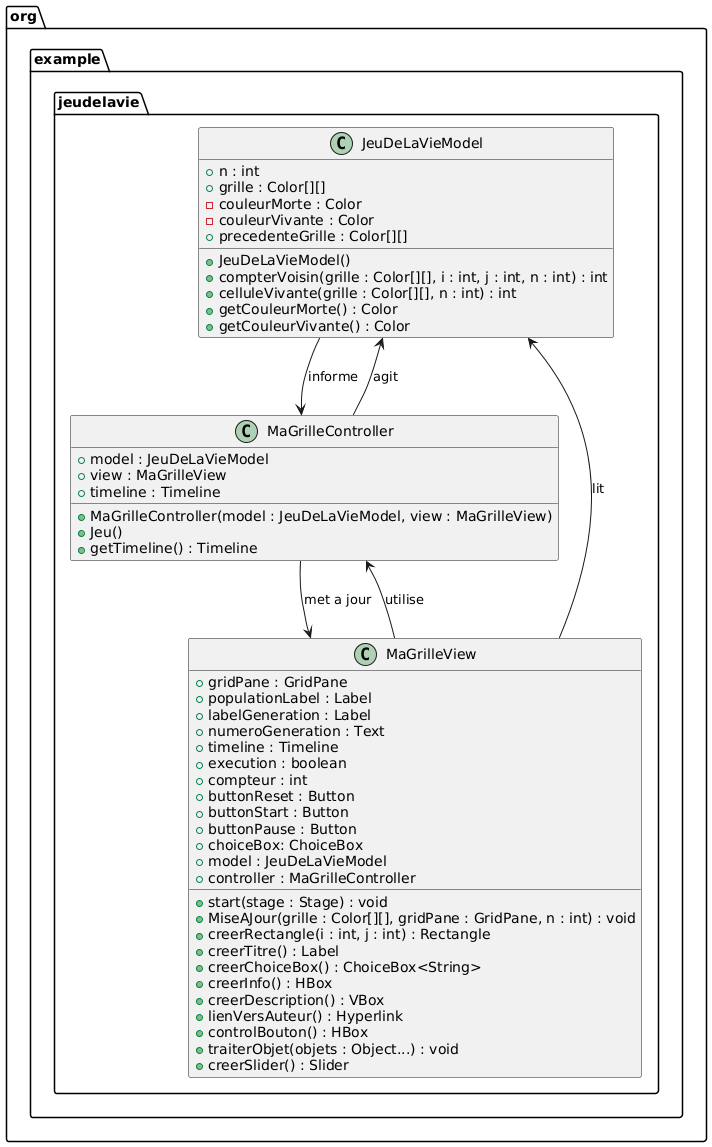
\includegraphics[width=0.9\linewidth]{Diagramme_classe_JeuDeJaVie.png}
        \caption{Le Diagramme des classes commenté}
    \end{figure}
    \subsection{Chaînes de traitement (comment les classes interagissent et pourquoi)}

Mon projet suit une structure inspirée du modèle MVC (Modèle - Vue - Contrôleur), afin de séparer la logique du jeu, l'affichage graphique, et la gestion du déroulement du jeu.

\begin{itemize}
    \item \textbf{La classe \texttt{JeuDeLaVieModel}} représente le \textbf{modèle}. Elle contient les données principales du jeu, notamment la grille (\texttt{grille}) et sa taille (\texttt{n}).
    
    \item \textbf{La classe \texttt{MaGrilleView}} représente la \textbf{vue}. Elle est responsable de l’affichage graphique. Elle possède la méthode \texttt{MiseAJour} qui permet de mettre à jour l'affichage à partir des données du modèle.
    
    \item \textbf{La classe \texttt{MaGrilleController}} représente le \textbf{contrôleur}. Elle fait le lien entre le modèle et la vue. Elle utilise le \texttt{Timeline} (animation JavaFX) pour actualiser le jeu automatiquement toutes les 500 millisecondes. À chaque intervalle, la méthode \texttt{Jeu()} est appelée, ce qui permet de transmettre les données du modèle à la vue pour mettre à jour l’affichage.
\end{itemize}
    \section{Expérimentations et usages}
    \subsection{Cas d'utilisation}
    \begin{itemize}
        \item \textbf{Simulation du Jeu :} L'utilisateur peut observer l'évolution de la grille en appuyant sur le bouton "Start", qui lance la simulation. La grille évolue automatiquement selon les règles du Jeu de la Vie.\\
        \item \textbf{Mettre en pause la simulation :} L'utilisateur peut mettre en pause le jeu en appuyant sur le bouton "Pause".\\
          \item \textbf{Réinitialiser la grille :} L'utilisateur peut vider la grille (mettre toutes les cellules en état mort) en appuyant sur le bouton "Reset".\\
         \item \textbf{Modification manuelle de la grille:} L'utilisateur peut cliquer sur les cellules de la grille pour les rendre vivantes ou mortes avant de démarrer la simulation.\\
         \item \textbf{Modification aléatoire de la grille:} L'utilisateur peut rendre les cellules vivantes de façon aléatoire en choisissant le motif "Aléatoire" du choicebox avant de démarrer la simulation.\\
         \item \textbf{Gestion de la vitesse:} L'utilisateur peut contrôler la vitesse de la simulation grace au slider.
    \end{itemize}
    \subsection{Quelques images de la simulation en cours}
    \begin{figure}[H]
        \centering
        \includegraphics[width=0.9\linewidth]{ecranTotal.png}
        \caption{Interface utilisateur du jeu}
    \end{figure}
    \begin{figure}[H]
        \centering
        \includegraphics[width=0.6\linewidth]{aleatoire.png}
        \caption{Cellules remplies avec le motif aléatoire}
    \end{figure}
    \begin{figure}[H]
        \centering
        \includegraphics[width=0.6\linewidth]{stable.png}
        \caption{Jeu à l'état stable}
    \end{figure}
    \begin{figure}[H]
        \centering
        \includegraphics[width=0.6\linewidth]{oxillant.png}
        \caption{Mouvement oscillatoire}
    \end{figure}
    \subsection{Résultats quantifiables}
    Le projet n'implique pas des calculs lourds, mais juste la fluidité de l'animation et la gestion de la grille qui doivent être efficaces. Les performances dépendent de la taille de la grille et de la fréquence des mises à jour (intervalle de 500 ms dans mon projet ci).\\
    \section{Conclusion}
    \subsection{Récapitulatif des fonctionnalités principales}
    \begin{itemize}
        \item Initialisation de la grille \\
        \item Simulation du jeu \\
        \item Interface utilisateur \\
        \item Animation 
    \end{itemize}
    \subsection{Propositions d’améliorations}
    \begin{itemize}
        \item \textbf{Optimisation des performances :} Améliorer l'efficacité de la mise à jour de la grille, notamment pour les grandes tailles de grille. \\
          \item \textbf{Personnalisation de la taille de la grille :} Permettre à l'utilisateur de choisir la taille de la grille au démarrage de la simulation. \\
            \item \textbf{Ajout d'autres motifs prédéfinis :} Ajouter la possibilité de charger des motifs connus du Jeu de la Vie (canon, vaisseaux , oscillateurs ...etc).
    \end{itemize}
    \section{Liens utiles}
    \begin{itemize}
      \item Page wikipedia de John H Conway: \href{https://fr.wikipedia.org/wiki/John_Horton_Conway}{John Horton Conway}\\
    \item  Page wikipedia du jeu de la vie: \href{https://fr.wikipedia.org/wiki/Jeu_de_la_vie}{Jeu de la vie}.
     \end{itemize}
    \section{Références}
    \begin{itemize}
    \item   Lien pour consulter la: \href{https://openjfx.io/}{ Documentation de JavaFX}\\
        \item   Page wikipedia du jeu de la vie: \href{https://fr.wikipedia.org/wiki/Jeu_de_la_vie}{Jeu de la vie}\\
        \item  Page dcode du jeu de la vie: \href{https://www.dcode.fr/jeu-de-la-vie}{dcode}\\
        \item Playlist de: EvoluNoob: \href{https://www.youtube.com/watch?v=I_bpcc6R338&list=PLrSOXFDHBtfGPyx7UHfsJtrdnpa_ix0ah}{Javafx-cours}\\
        \item Playlist de: LES TEACHERS DU NET: \href{https://www.youtube.com/watch?v=02SFViTyX4A&list=PLlxQJeQRaKDSlg_sOFKqBHvFsox2ZVWbs&pp=0gcJCV8EOCosWNin}{APPRENDRE JAVAFX}\\
        \item Je me suis inspiré de l'explication d'une partie de la video ci pour créer la grille cyclique (l'idée de faire modulo "taille de la grille" dans la méthode "compterVoisin" de la classe "JeuDeLaVieModel"): \href{https://youtu.be/NFeXmL_VxvA?t=3424}{Video- youtube}
    \end{itemize}
\end{document}